\documentclass{article}

\usepackage{a4wide}
\usepackage[dvipdfmx]{graphicx}
\usepackage{fancybox}
\usepackage{ascmac}
\usepackage{xspace}
%\usepackage{pdfpages}
\usepackage{pifont}
\usepackage{array}

\newcommand\st{\textsuperscript{st}\xspace}
\newcommand\nd{\textsuperscript{nd}\xspace}
\newcommand\rd{\textsuperscript{rd}\xspace}

\begin{document}

% cover letter
\begin{flushleft}
  2018-03-02\newline 
  Journal of Information Processing\newline
  Submission ID: 18-Y008e\newline
  Title: Component-Based mruby Platform for IoT Devices\newline
  Authors: Takuro Yamamoto, Takuma Hara, Takuya Ishikawa, Hiroshi Oyama, Hiroaki Takada, and Takuya Azumi\newline
\end{flushleft}

\textbf{Dear Editor and Reviewer,}\newline

We highly appreciate the insightful suggestions and detailed valuable comments on our paper.
The suggestions of the reviewers are very helpful for us and the suggestions are now incorporated in the revised paper as follows.
We have attached the last paper review and revised paper in our reply letter.
In the revised paper, newly added and modified sentences are written in the bold and red colored font so that the reviewers can easily find them.
We hope the editor and the reviewers will be satisfied with our replies to the comments and the revised paper.
\newline\newline

\begin{flushleft}
  Yours sincerely,\newline

  Takuro Yamamoto\newline
  Osaka University\newline
  Email address: t-yamamoto@hopf.sys.es.osaka-u.ac.jp\newline
\end{flushleft}

\clearpage

\section{Response to Meta-reviewer}
\begin{enumerate}

\item \begin{flushleft}
\textbf{Comment:}

Basically, the proposed framework seems to be useful.
However as the reviewers suggest, this paper is not sophisticated as a research paper including English.

\end{flushleft}

\begin{flushleft}
\textbf{Our reply:}

Thank you for the comments.
In order to reflect the comments of reviewers, we fixed abstract and introduction, and added requirements and evaluations such as the execution time and memory consumption of UDP (4.2) and TLSF+TECS (4.4).
Furthermore, we fixed our English in this paper by a native speaker in a proofreading company.
For more detail, please see our replies as follows.

\end{flushleft}


\end{enumerate}

\clearpage


\section{Response to 1\st reviewer}

\begin{enumerate}

\item \begin{flushleft}
\textbf{Comment:}

Please describe the relation between mruby and proposed framework clearly. I think that the developed component can be used as a normal TECS component without mruby. I cannot understand why the paper says "mruby." 
\end{flushleft}

\begin{flushleft}
\textbf{Our reply:}

Thank you for your suggestion.
The main contribution of this paper is to build a platform for IoT devices with high productivity using mruby.
We modified Abstract as follows. 

However, as the reviewer 1 mentioned, the proposed two functionalities, TINET+TECS and TLSF+TECS, can be applicable to various embedded systems because these frameworks are executed on TECS and not limited to mruby.
We added the following sentence in Section 6.

\begin{itembox}[|]{Abstract}
In this paper, we propose an extended mruby on TECS framework for its application in developing software for IoT devices, including sensors and actuators. Our proposed framework enables mruby programs to utilize Tomakomai Internetworking (TINET), a TCP/IP protocol stack specifically designed for use in embedded systems. Further, the proposed framework incorporates two component-based functions, i.e., a componentized TINET stack called TINET+TECS and a componentized Two-Level Segregate Fit (TLSF) dynamic memory allocator called TLSF+TECS.
\end{itembox}\\


\begin{itembox}[|]{Conclusion}
TINET+TECS and TLSF+TECS can be applicable to various embedded systems because these frameworks are executed on TECS and not limited to mruby.
\end{itembox}\\

\end{flushleft}


\item \begin{flushleft}
\textbf{Comment:}

Please describe requirements to implement these components for mruby or IoT system using TECS and explain its design associating with the requirements. 
\end{flushleft}

\begin{flushleft}
\textbf{Our reply:}

We added the requirements at the beginning of Section 2.
\begin{itembox}[|]{}
{\bf Requrements:} The requirements of the proposed mruby platform for IoT devices are defined as follows.
\begin{description}
    \item[R1:]
        TCP/IP functions can be utilized from mruby programs and the protocol stack can be easily configured for producivity since the network function is essential to the IoT systems.

    \item[R2:]
        Multiple mruby programs can run concurrently to improve productivity of software development.
        A thread-safe memory allocator is required to prevent the multiple mruby tasks from conflicting their memory.

\end{description}
\end{itembox}\\

\end{flushleft}

\item \begin{flushleft}
\textbf{Comment:}

The paper should explain evaluation of items described in contribution paragraph in the introduction. 

\begin{enumerate}
\item The authors said "Improve configurability," but there is no description of it in the evaluation section.  At least you should explain the proposed design can be used in typical cases. I cannot understand the validity of your design shown in Fig. 10 without them.  Please explain.

\item The paper also describes "Thread-safe memory allocator," but there is no evaluation of it. Please explain.
\end{enumerate}
\end{flushleft}

\begin{flushleft}
\textbf{Our reply:}

\begin{enumerate}
\item
    We added the new subsection (4.1) for the configurability evaluation.

\begin{itembox}[|]{4.1 Improved configurability}
As shown in Table 2, the code lines for modification were measured to demonstrate the improved configurability.
This demonstrated the ability to change the composition of the protocol stack with a small workload, confirming that the proposed framework improves the configurability.
\end{itembox}\\


\item
    We added evaluations of TLSF+TECS in Section 4.3.
    This section shows a comparison which two different applications are executed with two ways.
    One is to hold its own heap (TLSF+TECS), and the other is to utilize an exclusive control such as a semaphore.

\begin{itembox}[|]{4.4 Memory usage of RiteVMs by TLSF+TECS}
The proposed dynamic memory allocator, TLSF+TECS, executes multiple tasks without exclusive control concurrently because each TLSF component holds its own heap area.
The TLSF+TECS framework provides functionality to acquire statistical information describing dynamic memory usage.
Therefore, it is possible to analyze the operational status of the TLSF and GC on RiteVMs.
\ldots\ldots

% \begin{figure}[h]
    \centering
    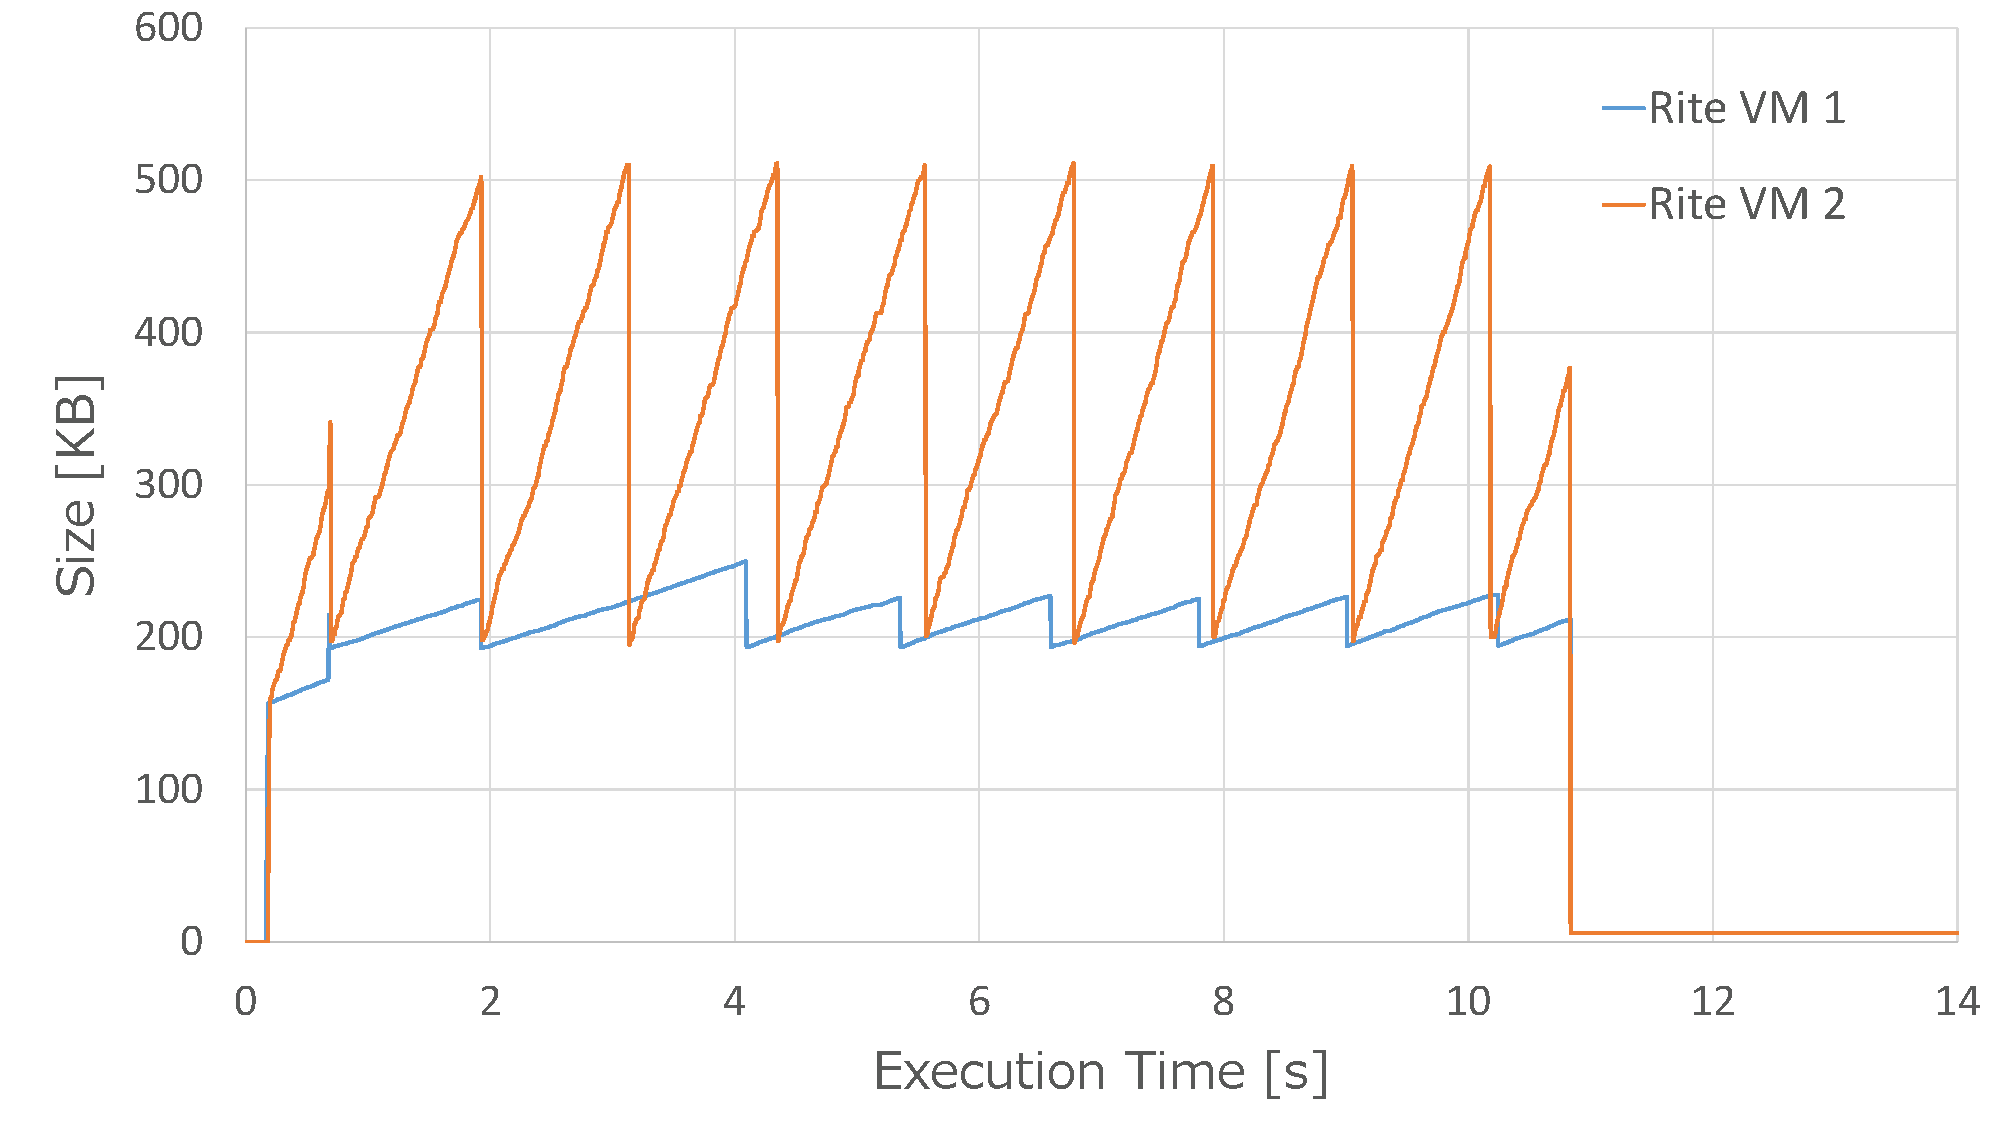
\includegraphics[width=8cm,clip]{../figure/EvaluationOfTLSFStatistics.pdf}
    % \caption{Memory usage of RiteVMs with TLSF+TECS}
    % \label{fig:EvaluationOfTLSFStatistics}
% \end{figure}

\end{itembox}\\

\end{enumerate}
\end{flushleft}

\item \begin{flushleft}
\textbf{Comment:}

Please add evaluation of typical usage pattern. The authors demonstrate execution time and memory usage using TCP only. 

\begin{enumerate}
\item Please evaluate execution time of connection time of TCP, UDP, and other supported protocol. If the overhead of them almost same as TCP, please discuss it. 

\item Please show memory usages under the typical configuration.
\end{enumerate}
\end{flushleft}

\begin{flushleft}
\textbf{Our reply:}

\begin{enumerate}
\item
    We added the execution times with UDP and discussed it.
    Note that we evaluated TCP and UDP which are supported by TINET.

\begin{itembox}[|]{4.2 Performance of TINET+TECS}
Conversely, we evaluated the execution times with UDP as shown in Fig. 29.
TINET+TECS can run at the same speed as TINET; therefore, the overheads of TINET+TECS are low.
\end{itembox}\\

\item
    We added the memory usage of only TCP, only UDP, and both TCP and UDP.

\begin{itembox}[|]{4.2 Performance of TINET+TECS}
\end{itembox}\\

\end{enumerate}
\end{flushleft}


\end{enumerate}

\clearpage

\section{Response to 2\nd reviewer}

\begin{enumerate}

\item \begin{flushleft}
\textbf{Comment:} 構成

タイトルとアブストラクトからは、TOPPERS 上にmrubyのプラットフォームを構築することで、IoTデバイスのproductivityを主張しているように思えますが、4章の評価は、execution time と memory consumptionになっており、こちらを主張したい点のようにも見えます。
主張したい点を明確にし、評価がその根拠となるように、Abstractを含む論文全体の構成とストーリー展開、タイトルを変更してください。

論文から、オリジナリティはTLSFとよぶダイナミックメモリアロケータを構築したことではないかと推測していますが、読み解くのは容易ではありません。
\end{flushleft}
\begin{flushleft}
\textbf{Our reply:}

productivityに関する評価(configurability)の節を新規に追加し,主張したい点が分かりやすいように変更しました.
execution timeとmemory consumptionの評価は,提案フレームワークを用いたオーバヘッドが小さいことを示しています.

\begin{itembox}[|]{4.1 Improved configurability}
As shown in Table 2, the code lines for modification were measured to demonstrate the improved configurability.
This demonstrated the ability to change the composition of the protocol stack with a small workload, confirming that the proposed framework improves the configurability.
\end{itembox}\\

\end{flushleft}

\begin{flushleft}
\textbf{1-(a):} AbstractとIntroduction

いずれもproposeが2回使われていますが、proposeは1回にまとめるべきで、提案は1つとし、含まれている特徴(問題点の解決策)を複数個記すようにした方が読みやすいです。「TINET+TECSおよびTLSF+TECSというフレームワークを提案する」というふうにまとめても良いとは思います。
また、問題点が一般的な背景ばかりが記されていて、提案方法が必要である問題点をAbstractとIntroductionから読み取ることができません。
シンプルに、解くべき問題点を列挙し、それに対応づく解決策を挙げるようにしてください。
\end{flushleft}
\begin{flushleft}
\textbf{Our reply:}

ご指摘ありがとうございます.
提案すべきは,「IoTデバイス向けのmrubyプラットフォーム」とし,それを実現するためにTINET+TECSとTLSF+TECSの2つの機能を組み込むという表現に修正を行いました(AbstractおよびIntroduction).
さらに,問題点と解決策が対応づくように,Introductionの貢献部分や要件(2章)を修正・加筆いたしました.

\begin{itembox}[|]{Abstract}
In this paper, we propose an extended mruby on TECS framework for its application in developing software for IoT devices, including sensors and actuators. Our proposed framework enables mruby programs to utilize Tomakomai Internetworking (TINET), a TCP/IP protocol stack specifically designed for use in embedded systems. Further, the proposed framework incorporates two component-based functions, i.e., a componentized TINET stack called TINET+TECS and a componentized Two-Level Segregate Fit (TLSF) dynamic memory allocator called TLSF+TECS.
\end{itembox}\\

\end{flushleft}

\begin{flushleft}
\textbf{1-(b):} 2. System Model

章立ての位置付けとして、この章では、IoTデバイスのproductivity向上についての要件や課題が記されていることを期待して読むのですが、TECSとmrubyの説明にとどまっています。論文は、新規性・有用性は何かを探しながら読むことが目的であり、開発に必要な知識を得ることは目的ではありません。新規性・有用性を主張するのに、必要な内容を記すようにしてください。
\end{flushleft}
\begin{flushleft}
\textbf{Our reply:}

2章システムモデルの冒頭に,提案フレームワークを実現するための要件を書き加えました.

\begin{itembox}[|]{}
{\bf Requrements:} The requirements of the proposed mruby platform for IoT devices are defined as follows.
\begin{description}
    \item[R1:]
        TCP/IP functions can be utilized from mruby programs and the protocol stack can be easily configured for producivity since the network function is essential to the IoT systems.

    \item[R2:]
        Multiple mruby programs can run in pallalel to improve producivity of software development.
        A thread-safe memory allocator is required to prevent the multiple mruby tasks from conflicting their memory.

\end{description}
\end{itembox}\\
\end{flushleft}

\begin{flushleft}
\textbf{1-(c):} 3章以降

AbstractおよびIntroductionを修正にともない、そのストーリーにあった内容にしてください。

\end{flushleft}
\begin{flushleft}
\textbf{Our reply:}

上で述べた通り,「IoTデバイス向けのmrubyプラットフォーム」を提案し,それを実現するために,2つの機能TINET+TECSとTLSF+TECSを組み込んだというストーリーにしました.
それに伴い,実現するための要件を加筆し,UDPの評価およびTLSF+TECSの評価を付け加えました.
\end{flushleft}

\begin{flushleft}
\textbf{1-(d):} 5. Related Work

MDDについてサーベイがありますが、execution time と memory consumptionを評価するならば、それと関連したサーベイをしてください。

\end{flushleft}

\begin{flushleft}
\textbf{Our reply:}

提案フレームワークの利点として,速い実行時間とコンフィグラビリティ性による小さいメモリ消費の2点を関連研究に加筆いたしました.

\begin{itembox}[|]{Related work}
mruby programs on TECS can be executed approximately 100 times faster than standard mruby programs [9].
That is, mruby programs can be executed at the same speed as C, which is faster than other scripting languages.

The proposed framework can configure the TCP/IP protocol stack with minimum set compared to the other platforms.
Therefore, the proposed framework can reduce memory consumption.
\end{itembox}\\

\end{flushleft}


\item \begin{flushleft}
\textbf{Comment:} 英語

理解できる英語ですが、論文誌の英語としては、全体的に、品質を向上させる必要があります。論文中に頻出する誤りとして、代表的な例は、下記が挙げられます。
abstractの二文目”To improve the productivity, ...”
この文章のTo…ではじまる文章ですが、懸垂分詞の誤りがあります。また、whichの修飾が適切でなく、主語と述語動詞の距離が長いです。以上のような問題点が散在しています。
\end{flushleft}

\begin{flushleft}
\textbf{Our reply:}

ご指摘ありがとうございます.
英文校正業者にネイティブ校正を依頼し,ご指摘頂いた点を含め,表現のミスや誤字・脱字の修正を行いました.
\end{flushleft}

\item \begin{flushleft}
\textbf{Comment:} 引用

・2.2冒頭

mruby is a light-weight implementation of the Ruby programming language complying to part of the ISO standard.
は、https://mruby.org/
の引用と思われます。引用番号を記すようにしてください。また、webの引用については、検索した日付をIPSJ論文誌の決まりに従い、入れるようにしてください。

mruby. Retrieved December 1, 2017 from https://mruby.org/
\end{flushleft}

\begin{flushleft}
\textbf{Our reply:}

ご指摘の通り,引用を追加いたしました.
IPSJ論文誌のサンプルを参考にWebの引用について修正を行いました.
\end{flushleft}

\item \begin{flushleft}
\textbf{Comment:} 

些細な誤りですが、Abstract の中程” The proposed framework enables that that mruby ” というふうにthat が重複しています。
上記の懸垂分詞やthatの重複などは、英語校正業者でなくても、メジャーな文法チェッカー程度で十分に修正できます。

\end{flushleft}

\begin{flushleft}
\textbf{Our reply:}

ご指摘ありがとうございます.
英文校正業者にネイティブ校正を依頼し,ご指摘頂いた点を含め,表現のミスや誤字・脱字の修正を行いました.
\end{flushleft}

\end{enumerate}

\end{document}

